\documentclass[twoside,11pt]{article}

\usepackage{aa228-jmlr2e}
\usepackage{amsmath}
\usepackage{graphicx}
\usepackage{lipsum}
\usepackage{listings}
\usepackage{url}
\usepackage{cleveref}
\usepackage{subcaption}
\usepackage{tikz}
\usetikzlibrary{calc}

\usepackage{enumitem}

\setlist[itemize]{noitemsep}  % or \setlist[itemize]{itemsep=0pt, topsep=0pt}

\begin{document}

\title{\texttt{trajectory\_utils}: Mathematical background}


%===========================================
\name{Stuart Johnson}
\email{stuart.g.johnson@gmail.com}

\maketitle

\tableofcontents

\section{Cartpoles}

\begin{figure}[h!]
\centering
\begin{minipage}{0.6\textwidth} % adjust width to taste
  \centering
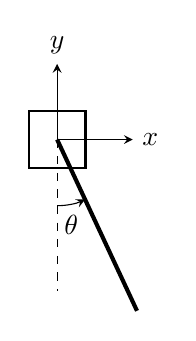
\begin{tikzpicture}[scale=1.2, >=stealth]

  % Parameters
  \def\cartW{0.6}     % cart width
  \def\cartH{0.6}     % cart height
  \def\L{2.0}         % pole length
  \def\thdeg{25}      % pole angle from downward vertical (for illustration)

  % Cart center & pivot
  \coordinate (cartcenter) at (0,0);
  \coordinate (pivot) at ($(cartcenter)+(0,\cartH/2)$);

  % Cart (small box)
  \draw[thick]
    ($(cartcenter)+(-\cartW/2,0)$) rectangle
    ($(cartcenter)+(\cartW/2,\cartH)$);

  % Axes from the pivot
  \draw[->] (pivot) -- ++(0.8,0) node[anchor=west] {$x$};
  \draw[->] (pivot) -- ++(0,0.8) node[anchor=south] {$y$};

  % Downward vertical from pivot (reference)
  \draw[dashed] (pivot) -- ++(0,-1.6);

  % Pole: angle measured from negative vertical toward positive x
  % So direction = -90 + \thdeg degrees
  \draw[line width=1.5pt]
    (pivot) -- ++({\L*sin(\thdeg)}, {- \L*cos(\thdeg)});

  % Mark angle theta at pivot (between downward vertical and pole)
  \begin{scope}
    \path (pivot) ++(0,-0.9) coordinate (downref);
    \draw[->]
      (pivot) ++(0,-0.7) arc[start angle=-90,
                             end angle={-90+\thdeg},
                             radius=0.7];
    \node at ($(pivot)+(0.15,-0.9)$) {$\theta$};
  \end{scope}

\end{tikzpicture}
\caption{\small Cart–pole system. The cart is actuated - by various means - and is constrained to move along $\pm x$. Objectives are to swing the pole up to vertical - and/or stabilize it there. The physical cart is actuated by a belt drive, and the pole is a steel rod.}
\label{fig:cartpole-diagram}
\end{minipage}
\end{figure}

\subsection{Equations of motion}

\subsection{Cart force control}

\subsection{Cart velocity servo control}

\subsection{The \texttt{cvxpy} experience}

\section{Differential Drive Control trajectories}

\subsection{Signed Distance Function (SDF) for obstacle avoidance}

\subsection{Differentiable SDF in pyTorch}

\subsection{The \texttt{cvxpy} experience}

% References
\bibliography{references}


\end{document}

